\chapter{ТЕСТИРОВАНИЕ СИСТЕМЫ АВТОМАТИЗАЦИИ УПРАВЛЕНИЯ ЖИЗНЕННЫМ ЦИКЛОМ ВЕБ-СЕРВИСА}
\label{cha:research}

\section{Проведение ручного тестирования}

Тестирование проводилось в браузере Safari Version 15.2 (17612.3.6.1.6).

Описание прохождения сценариев тестирования в порядке описания в плане:

\begin{enumerate}
    \item Для проведения данного сценария были рассмотрены следующие случаи:
    коммит не в основную ветку(не develop, testing или release) --- были составлена линия только из задач тестирования,
    коммит в основную ветку(develop, testing или release) --- были составлена линия из задач тестирования и задач создания релиза.
    Пример составленной линии представлен на Рисунке \ref{fig:qa-pipeline}, а пример пройденных автоматических тестов
    с генерированным файлами артифектов на Рисунке \ref{fig:qa-artifacts}.

    \begin{figure}[ht]
        \centering
        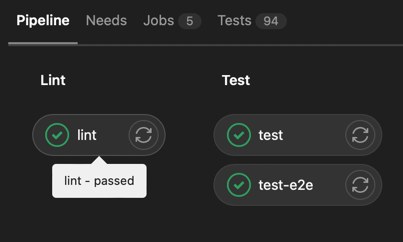
\includegraphics[scale=0.8]{figures/2}
        \caption{Линия тестирования в GitLab}
        \label{fig:qa-pipeline}
    \end{figure}

    \begin{figure}[ht]
        \centering
        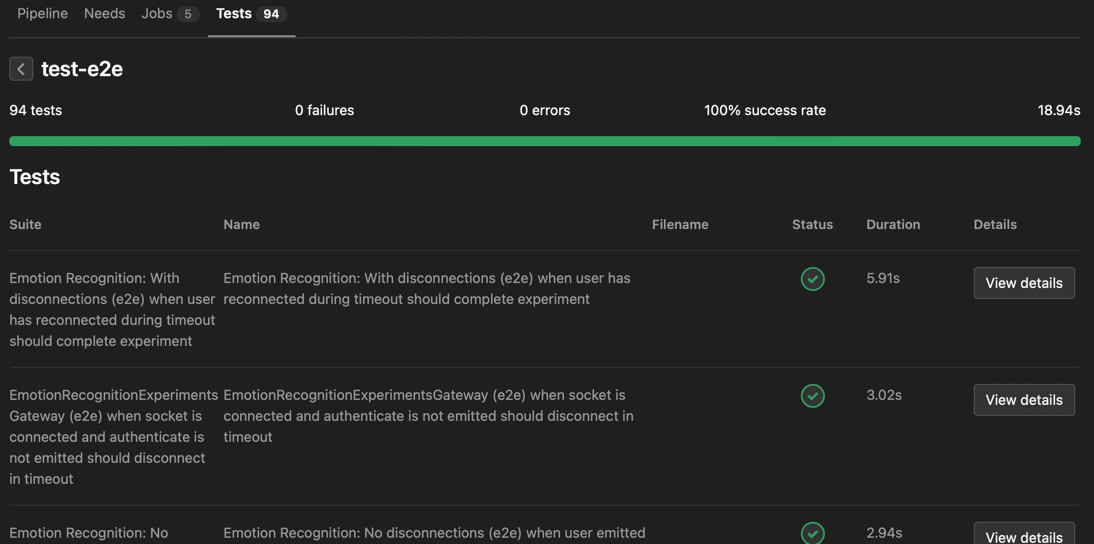
\includegraphics[scale=0.4]{figures/3}
        \caption{Артефакты тестирования в GitLab}
        \label{fig:qa-artifacts}
    \end{figure}

    \item Для проведения данного сценария были рассмотрены следующие случаи:
    создание релиза библиотеки --- для этого был произведён коммит в ветку develop, в ответ была составлена линия из задачи отправки библиотеки в регистр,
    а так же задач сборки Docker образа и обновления кластера;
    создание develop релиза --- для этого был произведён коммит в ветку develop, в ответ была составлена линия из задач тестирования,
    а так же задач сборки Docker образа и обновления кластера;
    создание testing релиза --- для этого был произведён мёрж коммит в ветку testing из ветки develop, в ответ была составлена линия из задач тестирования,
    а так же задач сборки Docker образа и обновления кластера;
    создание release релиза --- для этого был произведён мёрж коммит в ветку release из ветки testing, в ответ была составлена линия из задач тестирования,
    а так же задач сборки Docker образа и обновления кластера;

    Результаты тестирования представлены на скриншотах:

    \begin{figure}[ht]
        \centering
        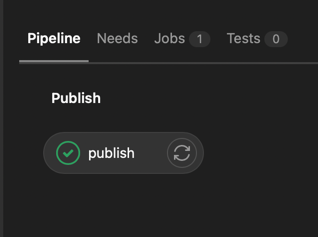
\includegraphics[scale=0.8]{figures/4}
        \caption{Загрузка библиотеки в хранилище}
        \label{fig:qa-library}
    \end{figure}

    \begin{figure}[ht]
        \centering
        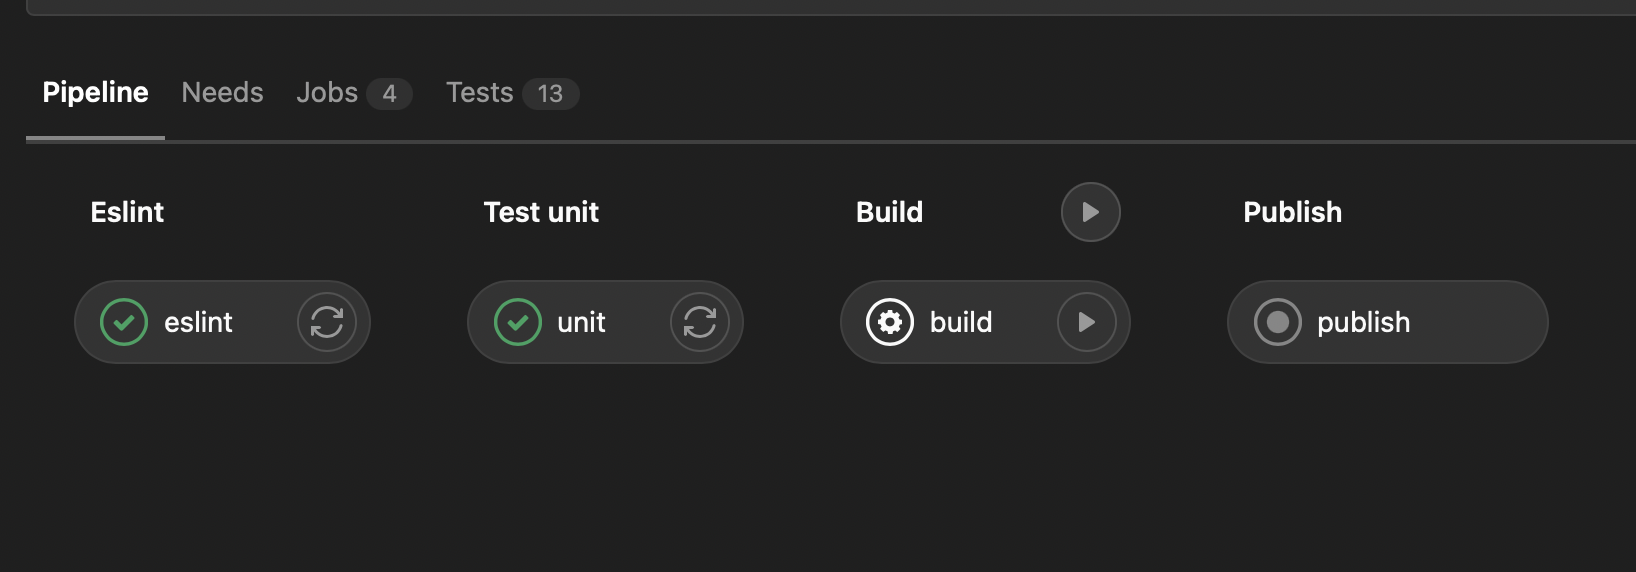
\includegraphics[scale=0.6]{figures/6}
        \caption{Срабатывает автоматизация тестирования, сборка по нажатию пользователя}
        \label{fig:qa-pipeline-trigger}
    \end{figure}

    \begin{figure}[ht]
        \centering
        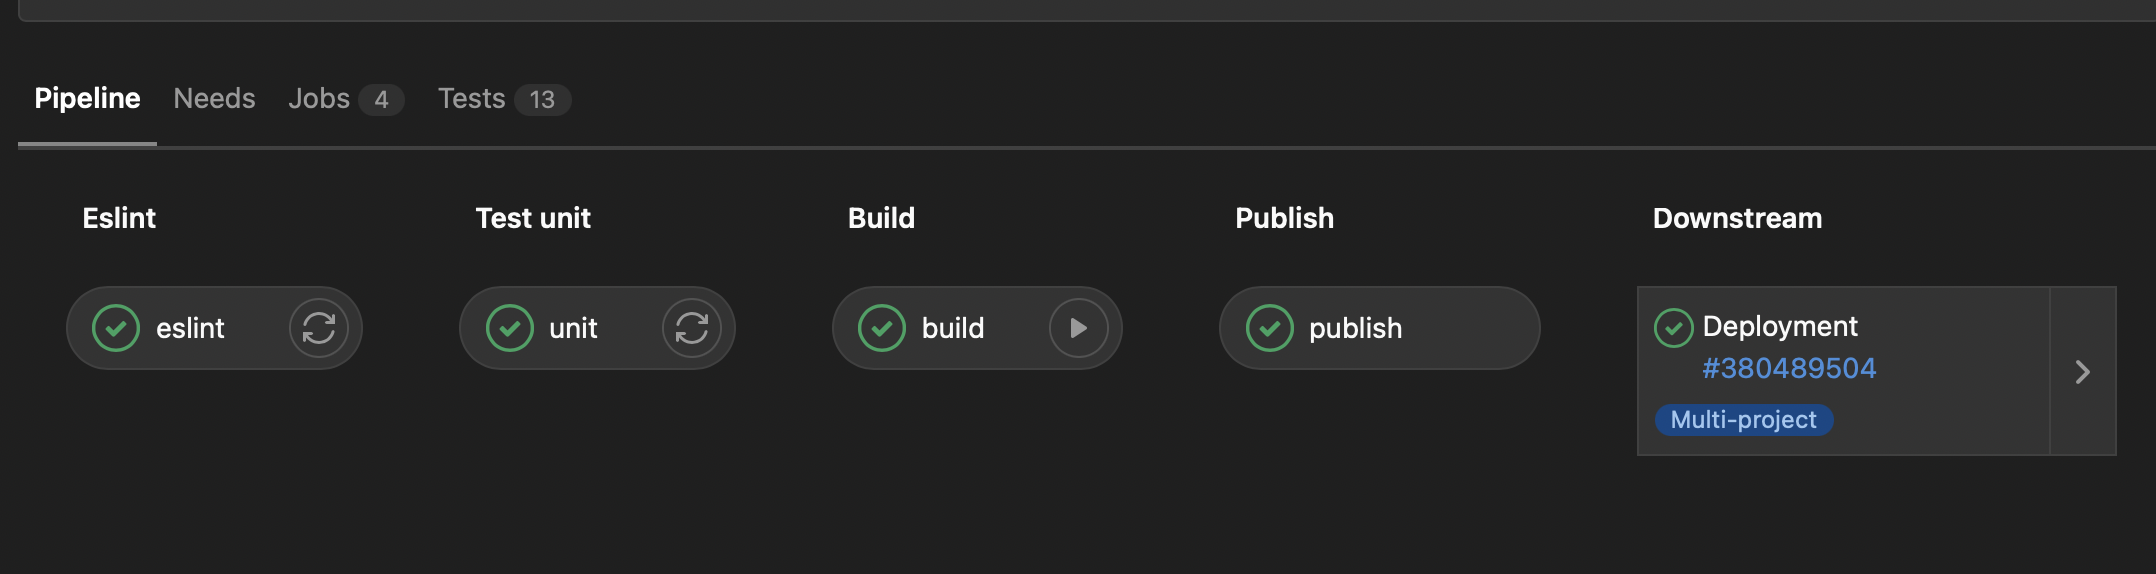
\includegraphics[scale=0.4]{figures/7}
        \caption{Успешное создание релиза}
        \label{fig:qa-release-creating}
    \end{figure}

    \item Для проведения данного сценария были рассмотрены следующие случаи:
    изменение количества сервисов api в окружении release --- были составлена линия только из задач тестирования,
    изменение количества сервисов web-client в окружении release --- были составлена линия только из задач тестирования,
    изменение системных ограничений сервиса api в окружении release --- были составлена линия только из задач тестирования.

    \begin{figure}[ht]
        \centering
        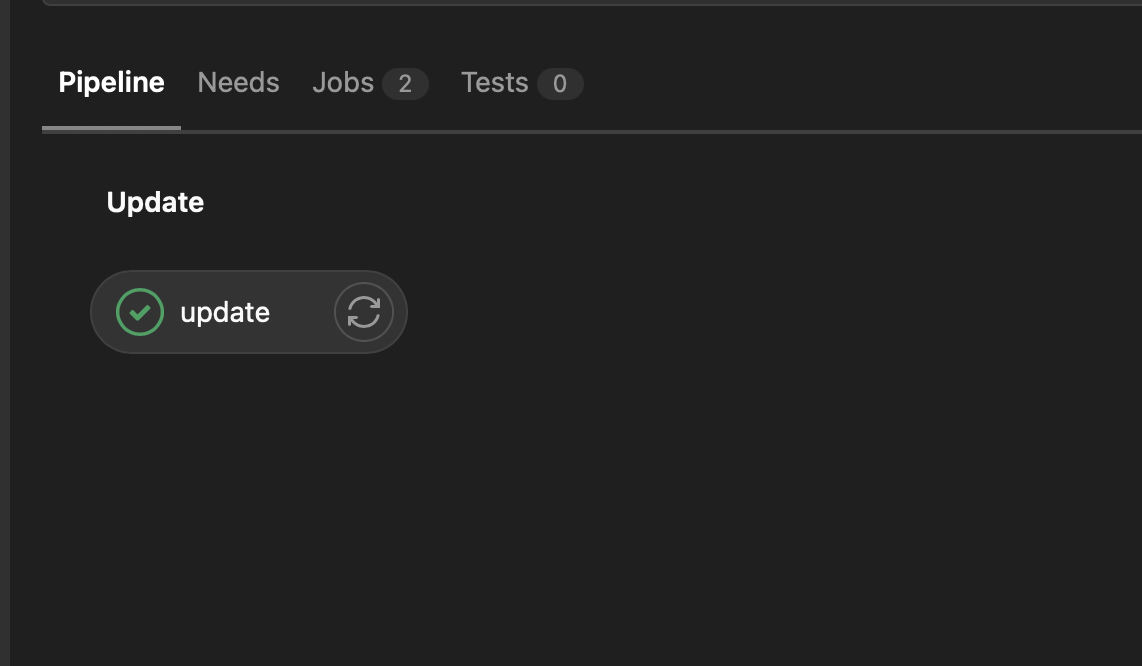
\includegraphics[scale=0.8]{figures/8}
        \caption{Применение конфигураций развёртки}
        \label{fig:qa-deploy}
    \end{figure}
    \item

    \begin{figure}[ht]
        \centering
        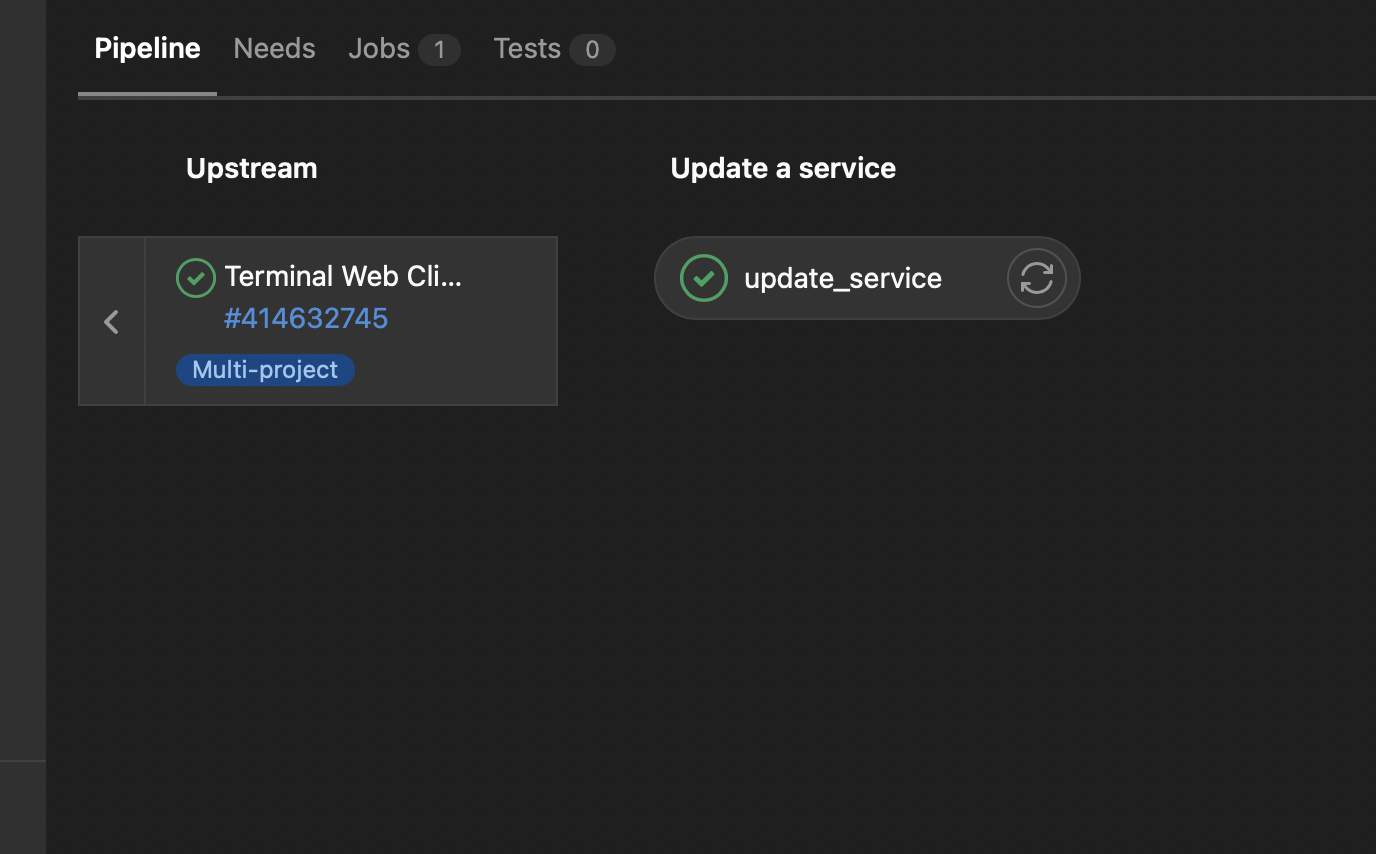
\includegraphics[scale=0.6]{figures/5}
        \caption{Применение конфигураций развёртки определенного сервиса компонента}
        \label{fig:qa-deploy-service}
    \end{figure}
\end{enumerate}

\section{Анализ результатов тестирования}

Результаты тестирования представлены в виде таблицы:

\begin{center}
    \begin{longtable}{|c|p{0.15\textwidth}|p{0.2\textwidth}|p{0.2\textwidth}|p{0.2\textwidth}|}
        \caption{Результаты тестирования}
        \label{tab:testing-res}
        \hline
        № & Название теста & Фактический результат & Ожидаемый результат & Комментарий                                                   \\
        \hline
        1 & Линия задач автоматизации тестироания  & Линии собираются правильно, задачи выполняются, артефакты предоставляются & Линии собираются правильно, задачи выполняются, артефакты предоставляются & - \\
        \hline
        2 & Линия задач релиза создания релиза  & Линии собираются правильно, задачи выполняются, веб-сервиса обновляется & Линии собираются правильно, задачи выполняются, веб-сервиса обновляется & Процесс создание релизов не самый простой  \\
        \hline
        3 & Линия задач управления развёрткой  & Веб-сервис правильно реагирует на изменение конфигураций развёртки & Веб-сервис правильно реагирует на изменение конфигураций развёртки & Требуется несколько минут на применение настроек \\
        \hline
    \end{longtable}
\end{center}

Все тесты пройдены успешно согласно плану, несмотря на небольшие проблемы с производительностью.

%%% Local Variables:
%%% mode: latex
%%% TeX-master: "rpz"
%%% End:
